\section{Kommunikation der Komponenten}
Die entwickelte Anwendung besteht mit einem Java-Service für die verwendete Wetter-API, der Complex Event Processing Engine und den Anwender-Clients aus drei Komponenten. Diese Komponenten müssen möglichst stark entkoppelt miteinander kommunizieren können. Durch eine starke Entkopplung wird erreicht ,dass die jeweiligen Komponenten keine Kenntnisse über vorhandene Schnittstellen oder die verwendete Programmiersprache besitzen müssen. Um dies zu realisieren, wird RabbitMQ als Message-oriented Middleware (MoM) eingesetzt. 
\subsection{RabbitMQ}\label{rabbitmq}
Bei RabbitMQ handelt es sich um einen auf Erlang basierenden OpenSource Message Broker, welcher Bibliotheken für alle gängigen Programmiersprachen wie Java, JavaScript, Swift und C\# anbietet. Dadurch wird die Kommunikation mit Android-, iOS- und Webapplikationen möglich. Durch die Verwendung von Queues und Topics wird die asynchrone Verteilung der Nachrichten ermöglicht. RabbitMQ verwendet als Standard das Messaging Protokoll AMQP, bietet aber Plugins für alternative Protokolle wie MQTT und STOMP. Da auch mobile Geräte zu den eingesetzten Komponenten gehören, wird das Protokoll MQTT eingesetzt, da dieses speziell für den Einsatz in Mobilgeräten entwickelt wurde. Die Kommunikation der einzelnen Komponenten erfolgt mit MQTT über Topics. Damit der Nachrichtenaustausch stattfinden kann, müssen sich die miteinander kommunizierenden Komponenten auf ein oder mehrere gemeinsame Topics einigen. Der Aufbau eines Topics ist mit REST-Schnittstellen vergleichbar und kann aus mehreren Topic-Leveln bestehen. Zusätzlich können beim Abonnement von Topics Platzhalter wie $+$ und \# eingesetzt werden. Diese funktionieren wie reguläre Ausdrücke und ersetzen im Falle des Platzhalters + eine einzelne Topic-Ebene und beim Platzhalter \# alle nachfolgenden Ebenen. Die Topics und mögliche Abonnements dieser Anwendung sind nachfolgend aufgelistet:
\begin{description}
\item[78467/today]\hfill \\ Abonnement des Wetters von Postleitzahl 78467 des heutigen Tages
\item[$+$/today]\hfill \\ Abonnement des Wetters aller verfügbaren Postleitzahlen des heutigen Tages
\item[78467/today/alert]\hfill \\ Abonnement der Wetterwarnungen für die Postleitzahl 78467
\item[$+$/weekly]\hfill \\ Abonnement der Vorhersage der nächsten Woche aller verfügbaren Postleitzahlen
\item[\#]\hfill \\ Abonnement aller verfügbaren Topics
\end{description}
Damit Daten durch einen Client versendet oder empfangen werden kann, muss er sich beim Verbindungsaufbau authentifizieren und für den Zugriff auf das entsprechende Topic autorisiert sein. Die Authentifizierung erfolgt über eine gewöhnliche Benutzername / Passwort - Abfrage. Um den Zugriff auf MQTT-Topics zu beschränken, ermöglicht RabbitMQ die Verwendung virtueller Hosts (vHosts). Durch diese erlangen die Nutzer nur Zugriff auf ein Topic, wenn sie für den vHost des Publishers autorisiert sind. 
\begin{figure}[htbp]
	\centering
	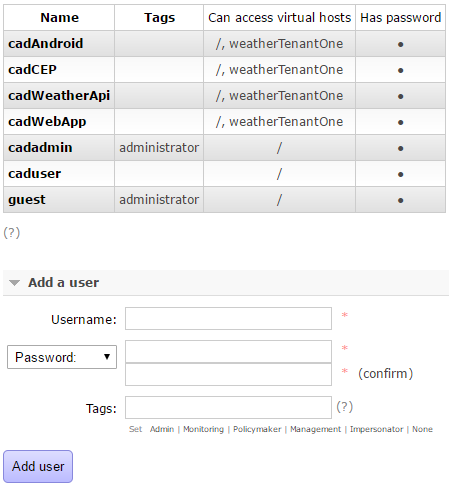
\includegraphics[width=0.5\textwidth]{Bilder/createUser.png}
	\caption{Administrationsmenü zur Benutzererstellung }
	\label{img:AdminCreateUser}
\end{figure}
Die Erstellung neuer Nutzer und die Verwaltung der Rechte erfolgt über unter anderem über das Management Plugin. In Abb. \ref{img:AdminCreateUser} ist ersichtlich, dass die User \textit{cadAndroid}, \textit{cadCEP}, \textit{cadWeatherApi} und \textit{cadWebApp} Zugriff auf den gemeinsamen vHost weatherTenantOne haben. Durch dieses Verfahren kann das gleiche Topic von mehreren Nutzern mit unterschiedlichen vHosts verwendet werden, ohne das sie die Nachrichten anderer vHosts des gleichen Topics lesen können. 
\begin{figure}[htbp]
	\centering
	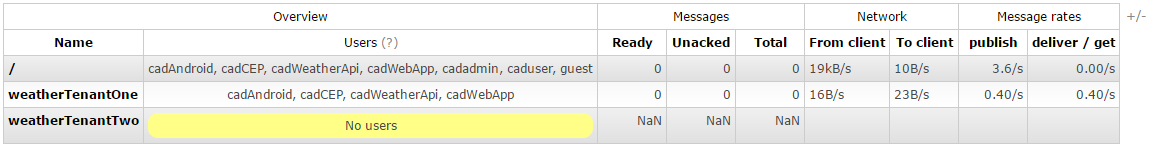
\includegraphics[width=1.0\textwidth]{Bilder/vHostsOverview.png}
	\caption{Übersicht über die virtuellen Hosts}
	\label{img:vHostOverview}
\end{figure}
Eine Übersicht über die einzelnen vHosts und die berechtigten Nutzer wird in Abb. \ref{img:vHostOverview} dargestellt. Diese zeigt noch einmal die erwähnte Zugriffsbeschränkung auf die vier Nutzer dieses Use-Cases sowie den aktuell verursachten Datentransfer der vHosts. Auf diese Weise erfüllt die Anwendung die Anforderung der Multi-Tenancy. Zusätzlich zum Management Plugin bietet RabbitMQ eine HTTP-Schnittstelle. Diese ermöglichen es dem Administrator zum einen über eine Kommandozeile in Verbindung mit Kommandozeilenprogrammen wie cURL (Client for URLs) die angebotenen Schnittstellen aufzurufen und dadurch unter anderem Nutzer anzulegen oder die Verbindungsraten der vHosts auszugeben und auszuwerten (vgl. https://pulse.mozilla.org/api/). Aufgrund der vorhandenen Schnittstellen bietet sich dem Entwickler die Möglichkeit, die Administration über eine eigene Applikation durchzuführen. 
\subsection{12 Faktor App}\label{12FactorApp}
In diesem Absatz wird dargestellt, ob und wie die Anforderungen umgesetzt wurden.

\begin{table}[!ht]
  \centering
    \begin{minipage}{17cm}
      \centering
      \begin{tabular}{*{3}{|l|p{3.0cm}|p{7.0cm}}}\hline
      \multicolumn{4}{|c|}{\cellcolor[RGB]{200,200,200}Validierung nach "12 Faktor APP"} \\\hline
     \textbf{ID}&\textbf{Anforderung}&\textbf{Validierungs Element}&\textbf{Erfüllt}\\\hline
     1.&Codebase&Andere Komponenten sind nur für das Testszenario da. Deployment verschiederner Versionen über Repo möglich&Ja\\
      \hline
     2.&Abhängigkeiten&Keine Abhängigkeiten zu anderen Komponenten&Nein\\
     \hline
     3.&Konfiguration&Konfigurationsdatei wird beim Start des Containers aufgerufen und schränkt den Gast-Zugang auf localhost ein. Credentials werden über Umgebungsvariablen im Amazon Container Service (ACS) gepflegt.&Ja\\
     \hline
     4.&Unterstützende Dienste&Keine unterstützenden Dienste vorhanden&Nein\\
     \hline 
     5.&Build, release, run& Könnte durch Jenkins verwaltet werden. Da die MOM keine regelmäßigen Update-Zyklen durchläuft, wurde darauf verzichtet.&Möglich,\- nicht aktiv\\
     \hline
     6.&Prozesse&Der Start des RabbitMQ wird durch das init-Skript im Dockerfile gesteuert. Dieses wird durch dem CMD-Befehl automatisch ausgerufen, so dass der Anwender nur den Task im ACS starten muss (ref{acs}).&Ja\\
     \hline
      7.&Bindung an Ports&Notwendige Ports werden über die EXPOSE-Befehle im Dockerfile deklariert. Das Mapping dieser Ports wird in den Container-Einstellungen von ACS definiert. &Ja\\
     \hline
      8.&Nebenläufigkeit&Die Skalierung kann über ACS erfolgen. ACS ist bereits hoch skalierbar und bietet dem Verwalter des Containers die Konfiguration der Skalierung an. So können Minimum- und Maximum-Tasks sowie eine gewünschte Anzahl an Tasks definiert werden. Die Anzahl der laufenden Tasks bestimmt die Anzahl der laufenden Instanzen. Im verwendeten Nutzungsplan von ACS ist eine Instanz im Mittel über einen Monat verteilt kostenlos verfügbar.&Ja\\
     \hline
      9.&Einweggebrauch&Der Container kann schnell stoppt und gestartet werden. Durch Probleme mit der Rabbitmq-eigenen Datenbank besteht dann allerdings die Gefahr, im laufenden Betrieb hinzugefügte Nutzer neu hinzufügen zu müssen, da diese bei Rabbitmq auf den Namen des Hosts gespeichert werden und sich dieser beim Neustart des Containers ändert. Ein Workaround wurde entwickelt, dieser aktualiert aber lediglich das Init-Skript und fügt diesem die Nutzer automatisch hinzu. Dadurch muss beim Neustart auch das Skript aktualisiert werden. &Teilweise\\
     \hline
     10.&Dev-Prod-Vergleichbarkeit&Containerisierung durch Docker (ref\{Docker}.&Ja\\
     \hline     
     11.&Logs&Das Docker-Image von Rabbitmq gibt die Log standardmäßig über Stdout (tty) aus&Ja\\
     \hline
     12.&Admin-Prozesse&Automatische Ausführung eines Skripts beim Containerstart&ja\\
     \hline
      \end{tabular}
   \caption{Validierung der CEP nach "12 Faktor APP"}\label{tab:AnforderungenCEP}
    \end{minipage}
\end{table}